\documentclass[a4paper]{article}

%% Language and font encodings
\usepackage{polski}
\usepackage[polish]{babel}
\usepackage[utf8x]{inputenc}
\usepackage[T1]{fontenc}
\usepackage{pdfpages}
\usepackage{indentfirst}
\usepackage{listings}
\usepackage{gensymb}

% Adjust penalties
\brokenpenalty=1000
\clubpenalty=1000
\widowpenalty=1000

%% Sets page size and margins
\usepackage[a4paper]{geometry}

%% Useful packages
\usepackage{amsmath}
\usepackage{graphicx}
\usepackage[colorlinks=true, allcolors=blue]{hyperref}
\usepackage{booktabs}
\usepackage{cancel}
\usepackage{tikz}

\usepackage{float}

\renewcommand\thesection{\arabic{section}.}
\renewcommand\thesubsection{\arabic{section}.\arabic{subsection}.}
\renewcommand\thesubsubsection{\arabic{section}.\arabic{subsection}.\arabic{subsubsection}.}

% The following commands are not supported in PSTricks at present
% We define them conditionally, so when they are implemented,
% this pgf file will use them.
\ifx\du\undefined
  \newlength{\du}
\fi
\setlength{\du}{15\unitlength}

\newcommand{\Vsp}[1]{\vtop to #1 {}}
\newcommand{\Hsp}[1]{\hbox to #1 {}}
\newcommand{\Small}{\scriptsize}

\title{Sprawozdanie nr 4}
\date{}

\begin{document}

\begin{center}
\begin{tabular}{|p{5cm}|l|l|l|}
    \hline
    Wydział \Vsp{5mm} & \multicolumn{1}{|l}{Dzień} &  & Nr zespołu\\
    & \multicolumn{1}{|l}{Data} &  & \\
    \hline 
    Nazwisko i Imię: & \Small Ocena z przygotowania  & \Small Ocena ze sprawozdania & \Small Ocena Końcowa \\
    1. & & &\\
    2. & & & \\
    3. & & & \\
    \hline
    \multicolumn{2}{|l|}{Prowadzący \Vsp{1cm}} & \multicolumn{2}{|l|}{Podpis prowadzącego} \\
    \hline
\end{tabular}
\end{center}

{\let\newpage\relax\maketitle}
\setcounter{secnumdepth}{2}
\setcounter{tocdepth}{2}

\section{Interferencja fal} %TODO może lepsza nazwa

\subsection{Opis ćwiczenia}

Celem ćwiczenia jest pomiar długości fal elektromagnetycznych metodami interferencyjnymi.
Wykorzystujemy do tego następujące przyrządy:
\begin{itemize}
\item interferometr Michelsona
\item interferometr Fabry-Perota
\item siatkę dyfrakcyjną
\end{itemize}
W eksperymentach zostały wykorzystane mikrofale oraz światło widzialne w postaci lasera o kolorze czerwonym.

\subsection{Wstęp teoretyczny}

\subsubsection{Interferencja}

Interferencja jest efektem nakładania się fal. W wyniku nałożenia może nastąpić wzmocnienie fali wypadkowej lub jej osłabienie.  Warunkiem trwałej interferencji fal jest ich spójność, czyli korelacja faz i równość częstotliwości. W przeciwnym wypadku może dość np. do dudnienia. %TODO może usunąć dudnienie
Fale powinny też posiadać identyczną częstość kołową w i mieć taką samą polaryzację.
Natężenia nakładających się fal opisane są wzorami
$$E_{1} = E_{01} sin( \omega t − kx )$$
$$E_{2} = E_{02} sin( \omega t − k ( x + \Delta ))$$

gdzie dla fali drugiej przebywa ona dodatkową drogę $\Delta$ która powoduje różnicę w fazach pomiędzy falami.

Podczas interferencji czyli dodaniu się fal otrzymujemy następującą zależność
$$E = E_{1} + E_{2} = E_{01} sin( \omega t − kx ) + E_{02} sin( \omega t − k x  − \phi )$$ gdzie $\phi =\frac{2\pi}{\lambda}\Delta$ - opisuje zmianę fazy spowodowaną przebyciem dodatkowej drogi optycznej.

Używane przez nas detektory reagują na średnią ilość energii padającej na jednostkę powierzchni w jednostce czasu. Energia fali jest proporcjonalna do kwadratu natężenia pola elektrycznego, zależność tą możemy otrzymać z poprzedniego wzoru wynosi ona:
$$E^2 = ( E_{1} + E_{2} ) = E_{01}^2 sin^2 ( \omega t − kx ) + E_{02}^2 sin^2 ( \omega t − kx − \phi ) + 2 E_{01} E_{02} sin( \omega t − kx ) sin( \omega t − kx − \phi )$$

Z czego po odpowiednich przekształceniach otrzymujemy 
$$E^2 = E_{01}^2 sin^2 (\omega t − kx ) + E_{02}^2 sin^2 ( \omega t − kx − \phi ) + E_{01} E_{02} [cos \phi − cos[ 2 ( \omega t − kx ) − \phi ]]$$

Mając powyższą zależność możemy wyznaczyć wcześniej wspomnianą średnią ilość energii na jednostę powierzchni
$$I = E^2 =\frac{E_{01}}{2} \frac{E_{02}}{2} + E_{01}E_{02} cos \phi$$

Ostatecznie otrzymując 
$$I = I_{1} + I_{2} + 2 \sqrt{I_{1} I_{2}} cos \phi$$

co dla przypadku przez nas badanego $I_{1} = I_{2}$ sprowadza się do związku
$$I = 2I_{0} + 2 I_{0} cos \phi$$

w zależności od kąta przesunięcia fazowego $\phi =\frac{2\pi}{\lambda}\Delta$ otrzymujemy $0$ lub $4 I_{0}$ bo $cos \phi$ odpowiednio osiąga wartości $-1$ lub $1$. Z powyższych rozważań wynikia ostatecznie że 
$\lambda = 2 \frac{\Delta}{2m+1} $ dla osłabienia oraz $\lambda = \frac{\Delta}{m}$ dla wzmocnienia.

\newpage

\section{Pomiary i obliczenia}
\subsection{Siatka dyfrakcyjna}
\begin{figure}[h]
\centering
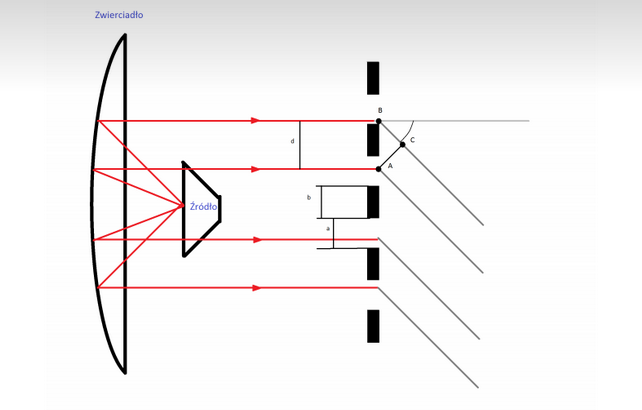
\includegraphics[scale=0.4]{siatka_dyfrakcyjna_rysunek.png}
\caption{Schemat układu pomiarowego dla siatki dyfrakcyjnej}
\label{siatka_dyfrakcyjna}
\end{figure}

\begin{figure}[h!]
\centering
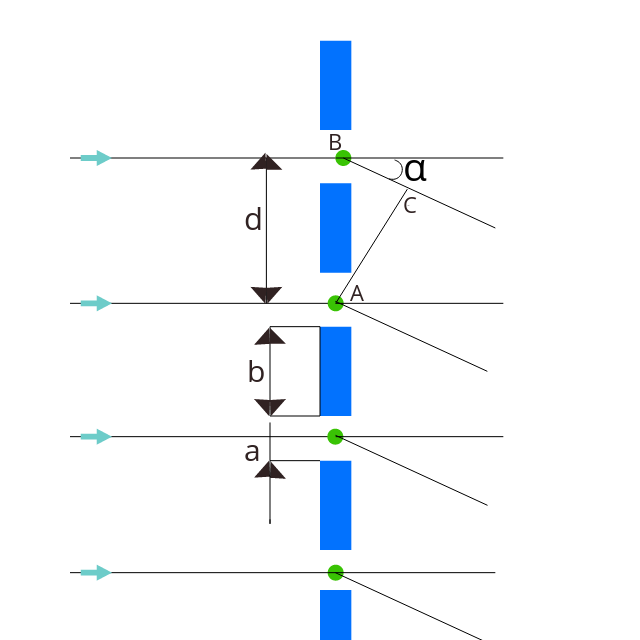
\includegraphics[scale=0.4]{siatka.png}
\caption{Schemat układu pomiarowego dla siatki dyfrakcyjnej}
\label{siatka}
\end{figure}


Do przeprowadzenia eksperymentu z siatką dyfrakcyjną posłużono się układem widocznym na rysunku \ref{siatka_dyfrakcyjna}. Źródło mikrofal które znajdowało się w odległości $\frac{1}{2}$ promienia krzywizny
zwierciadła wysyłało fale elektromagnetyczne które odbijały się od zwierciadła. Dzięki temu osiągaliśmy równoległe fale elektromagnetyczne. Następnie przechodziły przez szczeliny siatki dyfrakcyjnej
i zgodnie z zasadą Huyghensa były one wtórnymi źródłami fal kulistych które ze sobą interferowały dając minima oraz maksima sygnału obserwowanego na woltomierzu w miejsach o odpowiednich kątach względem siatki dyfrakcyjnej w których znajdował się odbiornik fal.
Na siatce dyfrakcyjnej dochodzi do powstania fal rozchodzących się kuliście, jeśli różnica dróg (wyznaczona przez długość pomiędzy punktami BC) widoczna na rysunku \ref{siatka} wynosi $$d sin \alpha_{m} = m \lambda$$ wówczas dochodzi do maksymalnego wzmocnienia fali wynikowej. Nasze pomiary polegały na wyznaczeniu kąta dla którego zachodzą te wzmocnienia, dzięki temu możemy określić długość fali. Podziałka na kątomierzu określającym położenie maksimum wynosiła $\Delta \alpha=1 \degree = 0.01745329 rad$  przyjmujemy niepewność eksperymentatora jako $\Delta \alpha_{e}=0.5 \degree = 0.008726646 rad$ stąd mamy że niepewność pomiarowa typu B wynosi
$$u_\alpha (\text{typ B}) = \sqrt{\frac{(\Delta \alpha)^2}{3} + \frac{(\Delta \alpha_e)^2}{3}} = \sqrt{\frac{(0.01745329)^2}{3} + \frac{(0.008726646)^2}{3}} rad \approx 0,011 \enskip \text{rad}$$


Otrzymano następujące wyniki:
\begin{table}[h!]
\centering
\begin{tabular}{rrr}
\toprule
Lp. &  $\alpha$ prawe (\degree) & $\alpha$ lewe (\degree)\\
\midrule
1 & 0 & 0\\
2 & 26 & 26\\
3 & 53 & 55\\
\bottomrule
\end{tabular}
\caption{Pomiary kątów dla maksimów wskazań woltomierza w eksperymencie z siatką dyfrakcyjną}
\label{pomiary_siatka}
\end{table}

Dokonaliśmy również pomiaru stałej siatki potrzebnej do wyznaczenia długości fali.
Metrówka którą wykonywaliśmy pomiar stałej siatki miała podziałkę $\Delta d=0.1 cm$ przyjmujemy niepewność eksperymentatora jako $\Delta d_e = 0.05cm$ skąd otrzymujemy niepewność typu B:
$$u_d (\text{typ B}) = \sqrt{\frac{(\Delta d)^2}{3} + \frac{(\Delta d_e)^2}{3}} = \sqrt{\frac{(0.1)^2}{3} + \frac{(0.05)^2}{3}} \approx 0.065 \enskip \text{cm}$$
Stała siatki wynosiła $d = \frac{89.1cm}{12} = 7.425cm$ by wyznaczyć ją z większą dokładnością należało określić łączną szerokość wielu szczelin i podzielić je przez ilość szczelin, dzięki temu niepewności polegające na niedokładnym przyłożeniu metrówki oraz niedokładnym odczytaniu końca ostatniej szczeliny możemy znacząco zmniejszyć.
Czyli uwzględniając niepewność otrzymujemy $d = 7.425(0.065)cm$
\\
Mając dwie powyższe niepewności przystępujemy do wyznaczenia niepewności dla pomiaru długości fali, obliczamy ją zgodnie ze wzorem
$$u_{\lambda} = \sqrt{(\frac{\partial \lambda}{\partial d})^2 \cdot u_d^2 + (\frac{\partial \lambda}{\partial \alpha})^2 \cdot u_{\alpha}^2} = \sqrt{sin^2 \alpha \cdot u_d^2 + d^2 \cdot cos^2 \alpha \cdot u_{\alpha}^2}$$

Kąty poszczególnych maksimów obliczamy jako średnia arytmetyczna z pomiaru lewego i prawego maksimum
$$\alpha_{n}=\frac{\alpha_{n}^L+\alpha_{n}^R}{2}$$

Ostateczne wyniki długości fali przedstawia tabela

\begin{table}[h!]
\centering
\begin{tabular}{rrrr}
\toprule
Lp &  kąt średni & długość fali [m] & niepewność pomiarowa\\
\midrule
1 & 0 & 0 & 0\\
2 & 26 & 0.03137 & 0.00079\\
3 & 54 & 0.03003 & 0.00071\\
\bottomrule
\end{tabular}
\caption{Długości fali w eksperymencie z siatką dyfrakcyjną}
\label{pomiary_michelson}
\end{table}


\subsection{Interferometr Michelsona - mikrofale}

\begin{figure}[h]
\centering
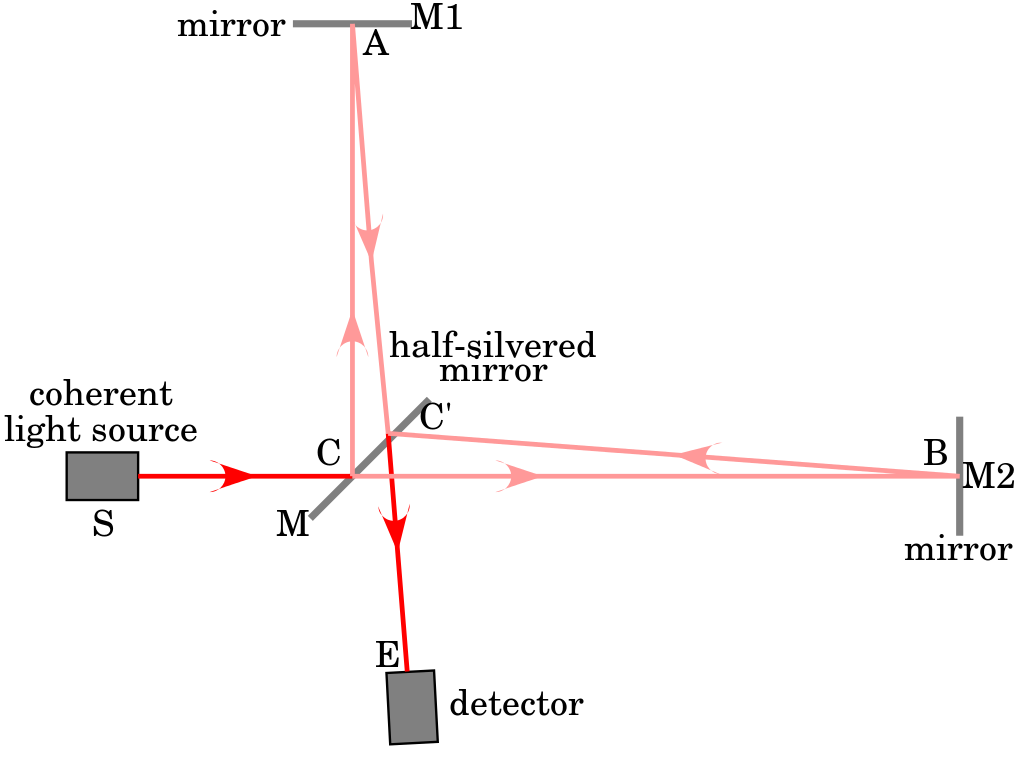
\includegraphics[scale=0.2]{Michelson_interferometer.png}
\caption{Schemat układu pomiarowego dla interferometru michelsona $https://upload.wikimedia.org/wikipedia/commons/thumb/d/d4/Michelson_interferometer_with_labels.svg/1024px-Michelson_interferometer_with_labels.svg.png$}
\label{michelson}
\end{figure}

 Wiązka mikrofal wychodzi ze źródła i pada na płytkę półprzepuszczlną. Połowa  wiązki odbija się od płytki pada na jedno ze zwierciadeł, odbija się i wraca tą samą drogą, przechodzi przez płytkę i pada na detektor.  Druga połowa wiązki przechodzi przez płytkę odbija się od drugiego zwierciadła i wraca tą samą drogą, odbija się od płytki, spotyka się z wiązką pierwszą w detektorze. Przesuwając jedno ze zwierciadeł zbadaliśmy ilość maksymalnych wzmocnień obserwowanych w detektorze oraz odległość na jakiej miało miejsce dane wzmocnienie.
By wyznaczyć długośc fali posłużyliśmy się następującym wzorem $\lambda = \frac{2 \sigma}{m}$
 Wyniki zestawiliśmy w poniższej tabeli. 
\newpage
\begin{table}[h!]
\centering
\begin{tabular}{rrrr}
\toprule
Lp. &  odległość ($cm$) & rożnica pomiędzy maksimami [m] & długość fali [m]\\
\midrule
1 & 2 & nie liczymy & nie liczymy\\
2 & 3.7 & 0.017 & 0.034\\
3 & 5.5 & 0.018 & 0.036\\
4 & 7.3 & 0.018 & 0.036\\
5 & 9.0 & 0.017 & 0.034\\
6 & 10.8 & 0.018 & 0.036\\
7 & 12.5 & 0.017 & 0.034\\
8 & 14.2 & 0.017 & 0.034\\
9 & 16.0 & 0.018 & 0.036\\
10 & 17.7 & 0.017 & 0.034\\
11 & 19.4 & 0.017 & 0.034\\
12 & 21.2 & 0.018 & 0.036\\
13 & 23.0 & 0.018 & 0.036\\
14 & 24.7 & 0.017 & 0.034\\
15 & 26.4 & 0.017 & 0.034\\
16 & 28.2 & 0.018 & 0.036\\
17 & 29.9 & 0.017 & 0.034\\
\bottomrule
\end{tabular}
\caption{Pomiary dla interferometru Michelsona}
\label{pomiary_michelson}
\end{table}

\begin{figure}[h!]
\centering
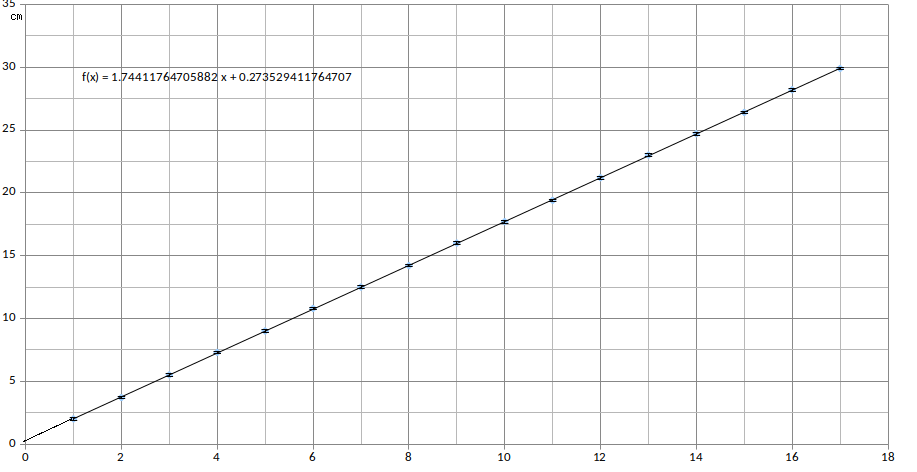
\includegraphics[scale=0.6]{michelson_micro.png}
\caption{Wykres różnicy dróg optycznych w zależności od numeru wzmocnienia}
\label{michelson}
\end{figure}

Obliczenia długości fali przeprowadzamy z użyciem metody najmniejszych kwadratów. Otrzymujemy współczynnik $a = 1.7441$ współczynnik b powinin być bliski 0 i tak jest w rzeczywistości, w naszych pomiarach wynosi on $b=0.2735$. Długość fali wynosi $\lambda = 3.49(0.02)cm$


\subsection{Interferometr Fabry-Perot}
Interferometr Fabry – Perota składa się z dwóch płytek, jedna z nich przepuszcza część promieniowania, a druga ma zdolność do odbijania. Płytki ustawiamy tak aby, powietrze pomiędzy płytkami tworzyło płaskorównoległą warstwę. Fale, które przez górną płytkę przedostają się do warstwy powietrza, ulegają wielokrotnym odbiciom od ścianek płytek. Jeśli na pierwszą płytkę pada wiązka fal, to z drugiej płytki wychodzi szereg równoległych wiązek. 
\\
\\
\\
Do pomiaru długości fal elektromagnetycznych wykorzystaliśmy drugi typ interferometru Fabry – Perota, gdzie jedna z płytek jest nieruchoma a druga jest zastąpiona zwierciadłem. Zmieniając położenie zwierciadła bada się różnicę dróg optycznych fal przy maksymalnych wzmocnieniach. Wyniki przedstawiliśmy w tabeli obok.

\begin{figure}[h!]
\centering
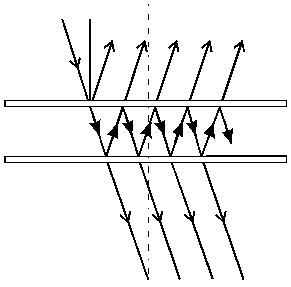
\includegraphics[scale=0.7]{fabry_perot.png}
\caption{Schemat układu pomiarowego dla interferometru Fabry-Perot $http://www.lodd.p.lodz.pl/~konrad/wyklad8/wyklad8/wyklad2.gif$}
\label{fabry_perot}
\end{figure}

Wyniki zestawiliśmy w poniższej tabeli. 

\begin{table}[h!]
\centering
\begin{tabular}{rrrrrrr}
\toprule
Numer maksimum & odległość (cm) \\
\midrule
0 & 9.0 \\
18 & 38.9 \\
\bottomrule
\end{tabular}
\caption{Wyniki pomiaru na interferometrze Fabry-Perot}
\label{pomiary_fabry_perot}
\end{table}

Długość fali obliczamy ze wzoru
$$\lambda = \frac{2}{r}cos \alpha (d_{m+r} - d_{m})$$
dla parametrów
$\alpha = 0, r = 18$
otrzymujemy $\lambda = 0.03322 m$
niepewności liczymy analogicznie do przypadku z siatką dyfrakcyjną otrzymując taką samą niepewność typu B dla metrówki (z powodu takich samych podziałek na obu linijkach) czyli
$$u_d (\text{typ B}) \approx 0.00065 \enskip \text{m}$$

Skąd możemy policzyć niepewność dla wyznaczenia długości fali. 
$$u_{\lambda} = \sqrt{(\frac{\partial \lambda}{\partial d})^2 \cdot u_d^2 } = \sqrt{\frac{2}{r}cos \alpha u_d^2}$$

po podstawieniu do wzoru otrzymujemy niepewność
$$u_{\lambda} = 0,00021 m$$
czyli ostatecznie długośc fali $$\lambda = 0.03322(0.00021)m$$

\subsection{Interferometr Michelsona - laser}
W ćwiczeniu interferometru Michelsona z laserem sam przyrząd został zbudowany w analogiczny sposób do wcześniej opisanego interferometru Michelsona z tym wyjątkiem że obecnie ruchami zwierciadła sterowaliśmy poprzez obroty śruby mikrometrycznej której podziałka miała dokładność
$0.01 mm$ i była ona zamontowana dodatkowo na dźwigni która umożliwiała zwiększenie dokładności ruchów 10 krotnie. Co też jest zbyt mało przy próbie bezpośredniego określenia długości fali. Lecz w naszym ćwiczeniu zastosowaliśmy metodę zliczania kolejnych maksimów i policzenia długości fali na podstawie różnicy wskazań na śrubie oraz ilości "miniętych" maksimów.
Mamy więc zależność
$$\lambda = ((\frac{d_{k} - d_{p}}{n}):10) \cdot 2$$

Wyniki przedstawiamy w tej tabeli:


\begin{table}
\centering
\begin{tabular}{rrrrrrr}
\toprule
Numer maksimum & odległość (mm) \\
\midrule
0 & 10.00 \\
110 & 10.33 \\
\bottomrule
\end{tabular}
\caption{Wyniki pomiaru na interferometrze Michelsona z laserem}
\label{pomiary_michelsona_laser}
\end{table}

Czyli otrzymujemy $\lambda = 660nm$ co jest zgodne z oczekiwaniami (światło czerwone ma długość fali około $700 nm$)


\section{Wnioski}
Najdokładniejszą metodą okazał się być interferometr Michelsona a najmniej dokładne pomiary występowały na siatce dyfrakcyjnej. Co ukazuje poniższa tabelka

\begin{table}[h!]
\centering
\begin{tabular}{rrrrrrr}
\toprule
Metoda & Wynik(cm) & Niepewność(cm) & Niepewność względna\\
\midrule
Siatka dyfrakcyjna & 3.07 & 0.08 & 0.026\\
Interferometr Michelsona & 3.49 & 0.02 & 0.005\\
Interferometr Fabry-Perot & 3.32 & 0.02 & 0.006\\
\bottomrule
\end{tabular}
\caption{Wyniki pomiaru na interferometrze Michelsona z laserem}
\label{porownanie_metod}
\end{table}

Wskazuje na to najmniejsza wartość niepewności. Niepewności pomiarowe wynikały przede
wszystkim z niedokładności przyrządów pomiarowych oraz niepewności odczytu wskazań urządzeń
przez eksperymentatora.

\end{document}
